\scanpage{107}
% Archive pencil foliation: 106.%
de Hodge), et par la condition qu\unsure{\deleted{t}e|\deleted{l}e|\deleted{e}t|\deleted{e}l} l'on a
\[
i_2=\overset{\handwritten{\rule{0.8em}{0.4pt}}}{i_1}\quad\text{i.e.}\quad i_2(\handwritten{\lambda})=\overset{\handwritten{\rule{2.2em}{0.4pt}}}{i_1(\handwritten{\bar{\lambda}}\rlap{\tikz[baseline=0pt,x=1em,y=1em]{\draw (-.05,.25)--(.65,.25);}})}\quad\text{pour tout}\quad\handwritten{\lambda\in}\underline{C}.
\]

Si à toute variété projective lisse $X$ sur $\underline{C}$ on associe sa cohomolo\deleted{g}gie rationelle $H^{\unsure{*|r|'}}(X,\underline{Q})=V$, de sorte que $V_{\underline{C}}=H^*(X,\underline{C})$ est isomorphe canoniquement (par la théorie de Hodge) à $H_{\mathrm{Hdg}}(X)=\handwritten{\coprod}H^q(X,\handwritten{\underline{\Omega}}^p_{X/\underline{C}})$, on voit qu'on trouve ainsi une pré-structure de Hodge sur $H^{\handwritten{*}}(X,\underline{Q})$, d'où un \inserted{\rlap{\handwritten{\begin{tikzpicture}[baseline=-.2ex,x=1em,y=1em]
\draw (-.3,-.5) .. controls (.4,.2) and (1.7,.05) .. (2,.7);
\end{tikzpicture}}}$\otimes$-}foncteur naturel de la catégorie d es motifs sur $\underline{C}$ dans la catégorie des pré-s\unsure{\deleted{c}t|\deleted{t}c}\unsure{\deleted{t}r|\deleted{r}t}\unsure{\deleted{r}u|\deleted{u}r|u}ctures de Hodge. La conjecture de Hodge \unsure{stándart|standart} équivaut à dire que ce foncteur est \uline{pleinement fidèle}, i.e. que l\deleted{\unsure{e|a}}'homomorphisme naturel qui va du groupe de Galois de Hodge précédent $G$ dans le groupe de Galois motivique (associé au \inserted{\rlap{\handwritten{\begin{tikzpicture}[baseline=-.2ex,x=1em,y=1em]
\draw (.4,-.6) .. controls (.35,-.1) and (1.6,.65) .. (1.8,1.3);
\end{tikzpicture}}}$\otimes$-}foncteur de Betti $H_{\mathrm{Bet}}$) est un épimorphisme. O\unsure{\deleted{\raisebox{.6ex}{U}}u|\deleted{u}\raisebox{.6ex}{U}} encore que pour toute catégorie \rlap{\handwritten{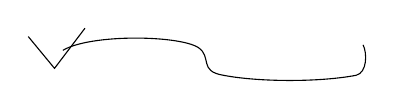
\begin{tikzpicture}[baseline=0pt,x=1em,y=1em]
\draw (-.25,.8)--(.7,-.35)--(1.8,1.1);
\draw (1,.3) .. controls (2,.9) and (5.2,.85) .. (5.9,.4) .. controls (6.4,.05) and (5.9,-.45) .. (6.8,-.6) .. controls (8.1,-.85) and (10.3,-.85) .. (11.6,-.6) .. controls (12,-.5) and (12,.2) .. (11.85,.5);
\end{tikzpicture}}}\inserted{$\underline{C}_o$} de motifs \inserted{de type fini} sur $\underline{C}$, désignant par $\underline{C}$ la \inserted{\rlap{\handwritten{
\begin{tikzpicture}[baseline=-.2ex,x=1em,y=1em]
\draw (-.3,.3) .. controls (.2,0) and (.35,-.3) .. (.5,-.7) .. controls (.5,.1) and (1.5,.7) .. (1.9,1.1);
\end{tikzpicture}}}$\otimes$-}catégorie de pré-s\unsure{\deleted{ct}\handwritten{t}|\deleted{\unsure{c|d}}t}ructures de Hodge engendrée par \deleted{celle-ci,} les $H_{\mathrm{Bet}}(M)$ pour $M\handwritten{\in}\operatorname{Ob}(\underline{C}_o)$, l'homomorphisme de groupes algébriques \begin{tikzcd}[cramped]G\arrow[r]&G_o\end{tikzcd} associé au foncteur de Betti-Hodge \begin{tikzcd}[cramped]\underline{C}_o\arrow[r]&\underline{C}\end{tikzcd} est un épimorphisme (i.e. surjectif sur les points à valeurs complexes, disons).


O\rlap{\raisebox{-.6em}{\handwritten{n}}}n appelle \deleted{structure} \uline{polarisation} d'une pré-structure de Hodge de poids $n$ la donnée d'un accouplement de préstructures de Hodge
\diagram{$\handwritten{\phi}:$\begin{tikzcd}[cramped]V\mathbin{\mathrm{x}}V\arrow[r]&\underline{Q}(n),\end{tikzcd}}
où $\underline{Q}(n)$ est l'espace vectoriel trivial $\underline{Q}$ sur $\underline{Q}$, avec $\underline{Q}_{\underline{C}}=\underline{C}$ muni d\unsure{\deleted{e}u|\deleted{u}e|\deleted{a}e|\deleted{e}a} \deleted{la}x bidegré $(n,n)$), ayant la propriété que la forme hermitienne correspondant\unsure{e|c} sur $V_{\underline{\unsure{\mathbb{C}|\deleted{G}C|\deleted{C}G}}}$,
\margin{\handwritten{\uline{\unsure{voir|Hdg|$\psi$|$\phi$}}}}
\[
\handwritten{\unsure{\psi|\deleted{\phi}\psi}}(x,y)=\handwritten{\phi}(x,\overset{\handwritten{\rule{0.5em}{0.4pt}}}{y})(\handwritten{i})^{p\handwritten{-q}}\quad\text{pour }x\text{ de bidegré }(p,\deleted{\unsure{n}}\handwritten{q}-p)
\]
soit définie positive. U\unsure{\deleted{u}n|\deleted{n}u|\rlap{\raisebox{.6ex}{n}}n}e \uline{structure de Hodge} est une préstructure de Hodge admettant une polarisation. Les structures de Hodge forment une \margin{\tikz[baseline=0pt,x=1em,y=1em]{\draw (0,0)--(.13,.12)--(.2,.3);}}sous-$\otimes$-catégorie de la catégorie des pré-structures de Hodge. La théorie de Hodge nous assure que le foncteur de Betti-Hodge sur la catégorie des

